%!TEX root = ../thesis.tex
\section{Computer-Generated Visualization}

\subsection{Augmented Workflow}
For presenters to narrate \"live\" over a video recording, we propose augmenting a typical workflow from capturing a screencast video; to rehearsing it and adjusting timings; and finally to live presentation of the demo video (Figure~\ref{fig:demowiz_workflow}).

DemoWiz first captures a screencast video and input events during a software demonstration from a user-defined rectangular region. Once the recording is done, DemoWiz analyzes the low-level event stream and transforms it into higher-level events such as mouse clicks, double-clicks, and drags. DemoWiz then allows presenters to edit the timing and notes while practicing their presentations with the presenter view equipped with an adjustable event timeline (Figure~\ref{fig:demowiz_teaser}a). Finally, presenters can give a live presentation using the same UI (i.e., presenter view) and show the audience view without visualization to the viewers.

\begin{figure*}[t]
  \centering
  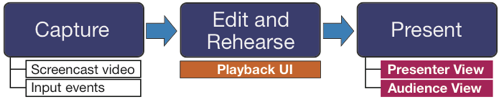
\includegraphics[width=\textwidth]{\demowiz/fig/demowiz_workflow}
  \caption{DemoWiz workflow: Presenters captures a software demonstration, edit the recording while rehearsing with our playback UI, and present the edited video to the audience using a presenter view.}
  \label{fig:demowiz_workflow}
\end{figure*}

% ---------------------------------------------------------------

\subsection{Visualizations}
To enable presenters to focus on their narration and the original video contents, DemoWiz augments the screencast recording by automatically overlaying simple glyphs.

\subsubsection{Input Event Glyphs}
DemoWiz overlays visual annotations of events on the screencast recording in a graphical way where the events happen.For example, in Figure~\ref{fig:demowiz_teaser}, the presenter clicks and drags the map view to the right. DemoWiz uses the following simple,distinctive glyphs to differentiate event types as Figure~\ref{fig:demowiz_glyphs} shows:

\begin{itemize}
  \itemsep -2pt
  \item Mouse click: a red circle with a radius of 20-pixels,
  \item Double-click: a green circle with a radius of 20-pixels,
  \item Mouse drag: a thin, orange line with a dot at the start point and an arrowhead at the end point,
  \item Mouse scroll: a thin, yellow line, 80 pixels long, with an arrowhead, and
  \item Keystrokes: text in blue.
\end{itemize}

At any given time during the video playback, DemoWiz shows the current event and the upcoming event on the video. We tried to show more than two events within a fixed time period in our initial prototypes. However, we noticed several issues. First, the view becomes too cluttered to understand at a glance, especially when the original video is visually complex. Second, it is not easy to convey the order of the events. Third, it is difficult to observe when multiple events are spatially close. Therefore, we provide minimum but essential events for recall.

\begin{figure*}[t]
  \centering
  
\includegraphics[width=\textwidth]{\demowiz/fig/event_types/types}
  \caption{DemoWiz visualizes input events in a graphical way. From the left to right we show a mouse click, double-click, a drag, a mouse scroll, and keystroke events. These glyphs are overlaid on the video recordings.}
  \label{fig:demowiz_glyphs}
\end{figure*}

% --------------------------------------------------

\subsubsection{Visual Guides to the Next Events}
In order to help guide the presenter's attention, DemoWiz overlays a motion arrow between the current and upcoming events on the demo video (Figure~\ref{fig:demowiz_teaser}c). This is inspired by storyboard design used in filming where an arrow effectively shows the movement of a camera or an actor in a single shot \cite{goldman2006schematic}. We expand the idea of guiding attention for a specific purpose: the arrow in DemoWiz shows the movement from one action (e.g., click a checkbox) to another action(e.g., click a button). By overlaying this motion arrow, the visualization matches the flow of a presenter's attention when they observe the video content.

Since the distance between two consecutive event segments vary, we created three visual designs to make sure the arrows are visible to lead a presenter's attention:

\begin{itemize}
  \itemsep -2pt
  \item For two events that are located far away (e.g., clicking an \"OK\" button after selecting a checkbox on a page), apply a\textit{straight} arrow (Figure~\ref{fig:demowiz_arrows}a).
  \item For events that are nearly at the same location (e.g., click the \"Next\" button twice to navigate a list of selections),apply a \textit{round} arrow that points to the current location (Figure~\ref{fig:demowiz_arrows}b).
  \item Otherwise, apply a \textit{curved} arrow (Figure~\ref{fig:demowiz_arrows}c).
\end{itemize}

\begin{figure*}[t]
  \centering
  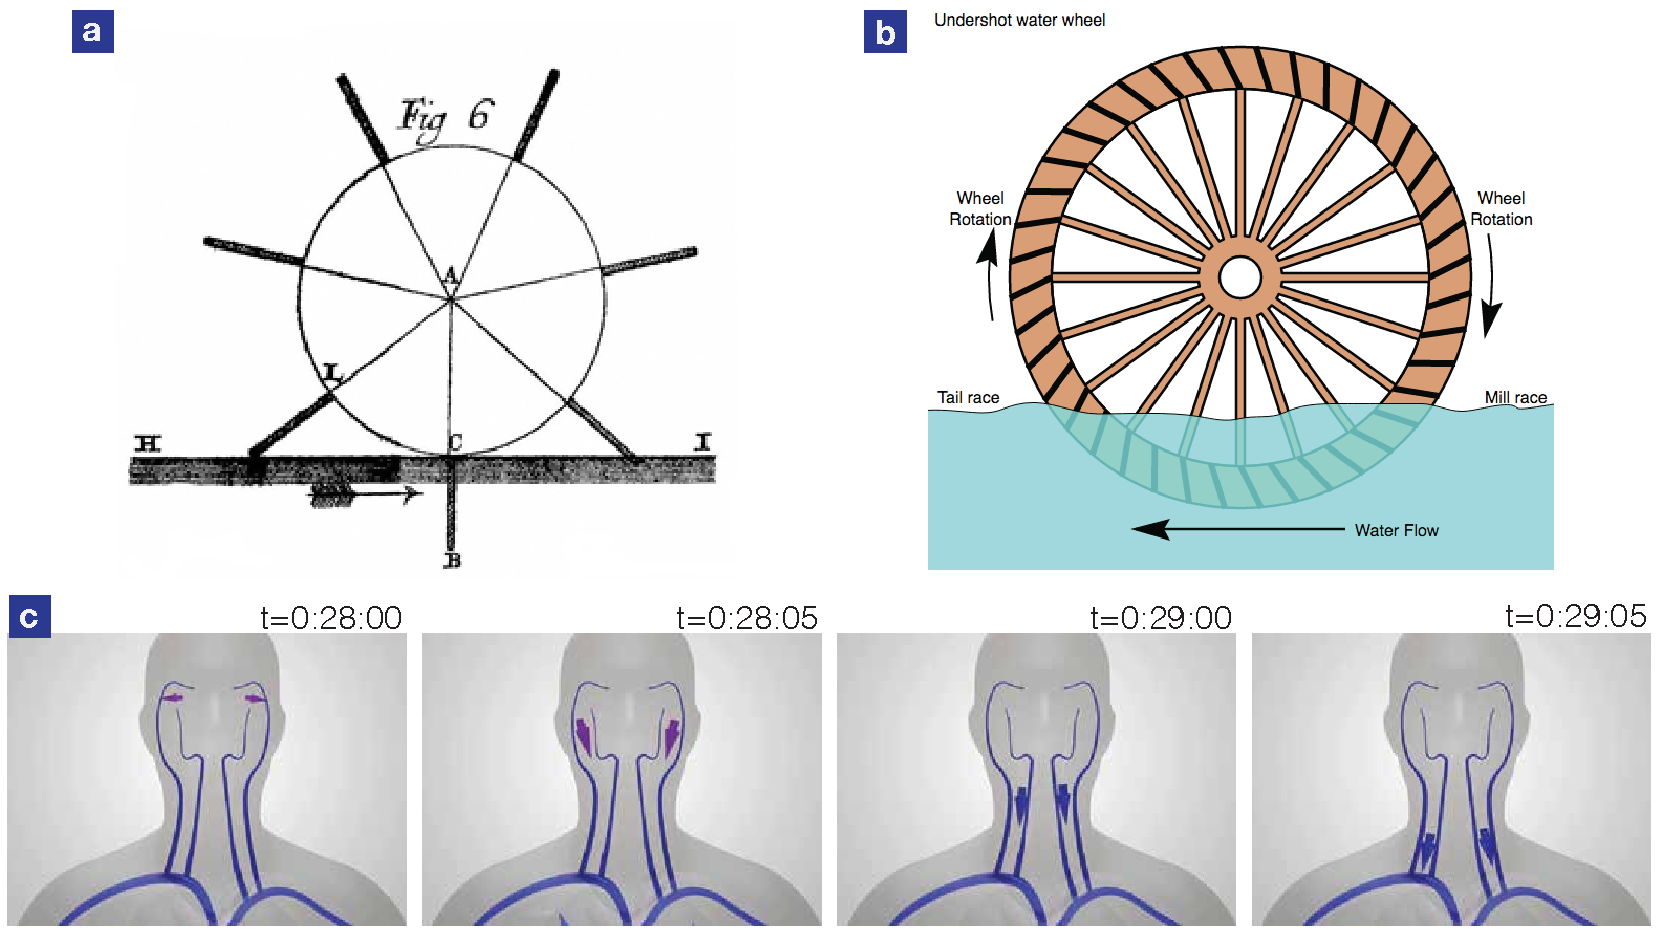
\includegraphics[width=\textwidth]{\demowiz/fig/arrows/arrows}
  \caption{Three types of motion arrows in DemoWiz that guide presenters to the next event of different distances at a (A) far, (B) nearly the same, and (C) near location.}
  \label{fig:demowiz_arrows}
\end{figure*}

% --------------------------------------------------

\subsubsection{Sense of Timing}
DemoWiz provides a sense of timing for an upcoming action so that presenters can adjust their narration. First, DemoWizembeds \textit{a progress bar} in the motion arrow to show relative time (Figure~\ref{fig:demowiz_teaser}c). The green bar shows the proportional time that has been passed before reaching the next event (Figure~\ref{fig:demowiz_timing} top). When a motion arrow is filled up with green, it fades away and guides the presenter to the next action. We were concerned that people may associate the length of an arrow to the length of time. Therefore, we also incorporated a \textit{countdown} visualization where circles will fade out in the last three seconds before the next action starts (Figure~\ref{fig:demowiz_timing} bottom) to convey absolute timing.

\begin{figure*}[t]
  \centering
  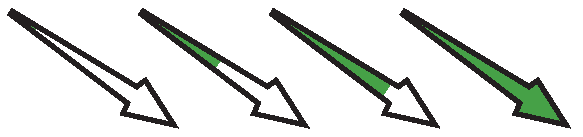
\includegraphics[width=\textwidth]{\demowiz/fig/progressbar/progressbar}
  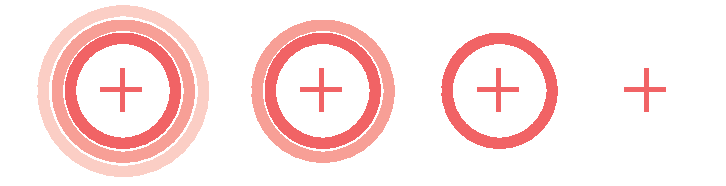
\includegraphics[width=\textwidth]{\demowiz/fig/countdown/countdown}
  \caption{A progress in time guides the presenter from the current event (left) gradually to the upcoming action (right) using relative timing with a progress bar (top) and absolute timing (bottom).}
  \label{fig:demowiz_timing}
\end{figure*}

% --------------------------------------------------

\subsubsection{Visualization Examples}
Figure~\ref{fig:demowiz_examples} presents examples of DemoWiz visualizations with four different systems. The glyphs effectively show the start and end points of mouse drags and the locations of mouse clicks. Motion arrows help direct the presenter's attention between events, such as start the end of the drag event to clicking a button (Figure~\ref{fig:demowiz_examples}a, ~\ref{fig:demowiz_examples}b), clicking between several options (Figure~\ref{fig:demowiz_examples}c), or selecting a specific slide after scrolling down (Figure~\ref{fig:demowiz_examples}d).

\begin{figure*}[t]
  \centering
  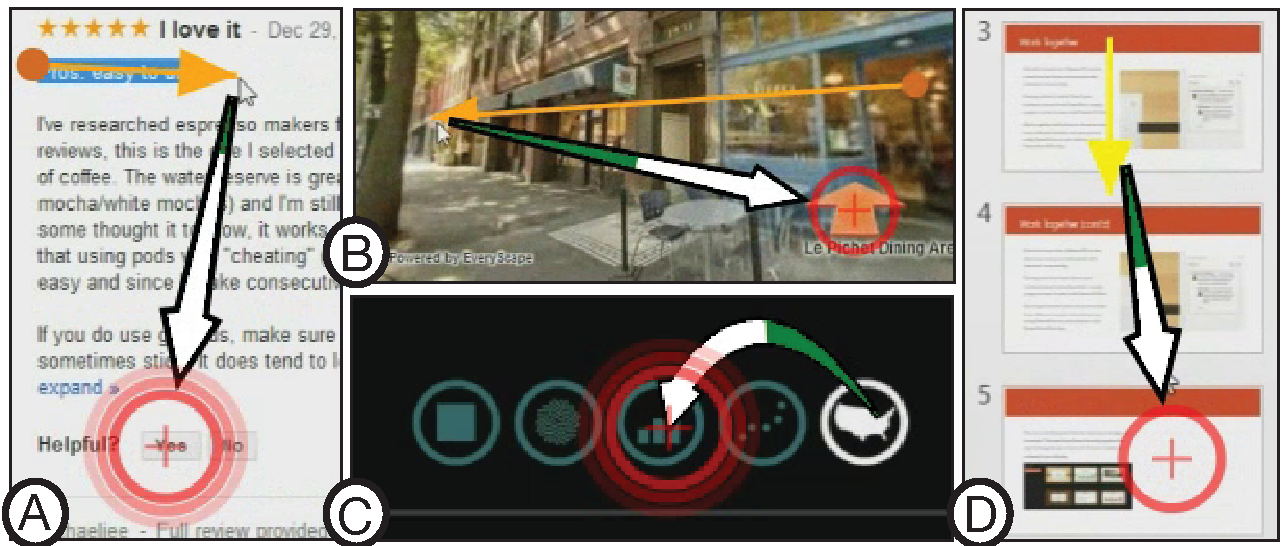
\includegraphics[width=\textwidth]{\demowiz/fig/examples/examples}
  \caption{Examples of DemoWiz visualizations with four different systems and input event sequences.}
  \label{fig:demowiz_examples}
\end{figure*}

% ---------------------------------------------------------------

\subsection{Lightweight Editing During Rehearsal}
During rehearsal for their demonstration, presenters can modify the video timing and add reminder notes for their narration. DemoWiz shows the type and length of each event in a sequence in a timeline (Figure~\ref{fig:demowiz_teaser}a). Each segment is shown as a block whose width indicates its length in time. To simplify the timeline and avoid fine-grained adjustment,lengths of event blocks are rounded to the second. Presenters can modify the playback speed of a segment by dragging the boundaries of a segment on the timeline. For example, presenters can speed up to shorten long text inputs, and slowdown for fast mouse drag inputs that select multiple objects.

Sometimes a change in the playback speed may result in an awkward effect that is noticeable to the audience, especially when showing a UI transition. Therefore, DemoWiz supports two special time control markers to enable breaks in the narration. Presenters can add an adjustable \textit{pause} segment, at which the system will pause at the last frame of the previous segment for the specified length of time. If presenters prefer full control on pause length, a \textit{stop} marker ensures the video stays paused at the last frame of the previous segment and will not proceed until presenters manually resume the playback of the video.DemoWiz enables presenters to add a short text note (such as the reminder \iquote{Move and zoom...} in Figure~\ref{fig:demowiz_teaser}) so that they could remind themselves of upcoming actions at a higher level. The note can be positioned manually at any location on a video so that it does not block important video content, and will be shown for 3 seconds before the associated event.For every edit that is associated with time changes (including playback speed and pauses), DemoWiz computes and updates the total presentation time as well as updating the progress bar and countdown to provide accurate timing.

% ---------------------------------------------------------------

\subsection{Presenter View}
During presentation, DemoWiz shows two views in separate windows. Presenters can observe visualizations using the presenter view, while the audience will see the audience view with a full-screen video that has no enhanced information. DemoWiz synchronizes the videos in both views based on presenters’ editing decisions to ensure the same playback speed and time. As with a conventional video player, presenters can control the video, to pause and play at any time. In addition, when a video is paused (or stopped), presenters can hover the mouse over the demo video in the presenter view to point out an important area, as many presenters currently do in a live demo. DemoWiz then simulates and synchronizes a mouse cursor in the audience view to help the audience follow the demonstration.

% ---------------------------------------------------------------

\subsection{Implementation Details}
During recording, DemoWiz captures the screen within a specified region and logs low-level system input data with\textit{timestamps} (with an accuracy of 0.1 seconds) from the operating system, including:

\begin{itemize}
  \itemsep -2pt
  \item \textit{Mouse events} (mouse downs, mouse ups, and mouse wheel movements) and their \textit{positions} (in x-y coordinates relative to the screen-captured region).
  \item \textit{Key-press events} (keyboard input).
\end{itemize}

Once presenters finish their demonstrations, DemoWiz analyzes the low-level event stream and transforms it into high-level event metadata. For mouse events, we pair each mouse down and up into mouse \textit{clicks}, \textit{double-clicks}, or \textit{drags}. We group any consecutive mouse wheel events within a time threshold of 2 seconds to one \textit{scroll} event and any key-press events within the same threshold to one \textit{keystroke} event(e.g., combine keys d-o-w-n-t-o-w-n to \"downtown\"). For each high-level event, we log the \textit{start} and \textit{end time} (timestamps of the first and the last low-level event).

Based on the start and end times of these high-level events, DemoWiz segments the screencast video recording into \textit{event segments}. Any gap between two consecutive input events is marked as an \textit{inactive segment}, which may include mouse hovering, UI transitions of the demo system, or static frames with no visual changes. DemoWiz adjusts the boundaries of these event segments to avoid any short visual effect that cannot be observed. DemoWiz examines segments in a linear order to ensure each segment lasts at least \textit{t}\textit{\textsubscript{min}} seconds long,which is set as one second based on our early testing. For an event segment \textit{S}\textit{\textsubscript{i}} of time (\textit{t}\textit{\textsubscript{start}},\textit{ t}\textit{\textsubscript{end}}) that\textit{t}\textit{\textsubscript{end }}\textit{$-$t}\textit{\textsubscript{start}} {\textless}\textit{t}\textit{\textsubscript{min}}, DemoWiz expands 0.5 second forward and backward if\textit{S}\textit{\textsubscript{i-1}} and \textit{S}\textit{\textsubscript{i+1}} are inactive. If the adjusted\textit{S’}\textit{\textsubscript{i-1}} and \textit{S’}\textit{\textsubscript{i+1}}\textit{ }are shorter than\textit{t}\textit{\textsubscript{min}}, DemoWiz merges it to the shorter neighbor segment. Currently, DemoWiz does not analyze these inactive segments, but techniques including computer vision and video analysis \cite{Banovic:2012kd,chi2012mixt} can be applied for finer segmentation.

The capturing program is implemented in C\#. Two APIs were used: 1) the Windows Event Log API for mouse and keyboard hooks and 2) the Expression Encoder 4 API for screen recording running on Microsoft Windows 7. The recorded metadata(stored in a JSON object) and screencast video (in MP4) are read by the Presenter UI, which is implemented using standard Web technologies, including HTML5, CSS3, JavaScript, and jQuery. In particular, the visualization is rendered on the canvas element on top of the video object on the fly based on the video playback time. The audience view is generated by the main browser window of presenter view for video control.
